\documentclass{article}

\usepackage[spanish]{babel}
\usepackage{listings}
\usepackage{color}
\usepackage[numbers,sort&compress]{natbib}
\usepackage{graphicx}
\usepackage{subfigure}
\usepackage{url}
\usepackage{amsmath}
\usepackage{hyperref}
\usepackage[top=15mm, bottom=40mm, left=15mm, right=15mm]{geometry}
\setlength{\parskip}{2mm}
\setlength{\parindent}{0pt}

\setlength{\parskip}{2mm}
\setlength{\parindent}{0pt}
\definecolor{blue}{rgb}{0,0.6,0}
\definecolor{gray}{rgb}{0.3,0.3,0.3}
\definecolor{orange}{rgb}{0.8,0.4,0}
\definecolor{mostaza}{rgb}{0.9,0.8,0.1}

\lstset{ %
  language=R,                     % the language of the code
  basicstyle=\footnotesize,       % the size of the fonts that are used for the code
  numbers=left,                   % where to put the line-numbers
  numberstyle=\tiny\color{gray},  % the style that is used for the line-numbers
  stepnumber=1,                   % the step between two line-numbers. If it's 1, each line
                                  % will be numbered
  numbersep=5pt,                  % how far the line-numbers are from the code
  backgroundcolor=\color{white},  % choose the background color. You must add \usepackage{color}
  showspaces=false,               % show spaces adding particular underscores
  showstringspaces=false,         % underline spaces within strings
  showtabs=false,                 % show tabs within strings adding particular underscores
  frame=single,                   % adds a frame around the code
  rulecolor=\color{black},        % if not set, the frame-color may be changed on line-breaks within not-black text (e.g. commens (green here))
  tabsize=2,                      % sets default tabsize to 2 spaces
  captionpos=b,                   % sets the caption-position to bottom
  breaklines=true,                % sets automatic line breaking
  breakatwhitespace=false,        % sets if automatic breaks should only happen at whitespace
  title=\lstname,                 % show the filename of files included with \lstinputlisting;
                                  % also try caption instead of title
  keywordstyle=\color{orange},      % keyword style
  commentstyle=\color{blue},   % comment style
  stringstyle=\color{mostaza},      % string literal style
  escapeinside={\%*}{*)},         % if you want to add a comment within your code
  morekeywords={*,...}            % if you want to add more keywords to the set
} 

\author{1445183}
\title{Práctica 4: Diagramas de Voronoi}
\date{\today}

\begin{document}

\maketitle

\section{Intoducción}
Se le llama diagrama de Voronoi a la representación de divisiones de un plano en regiones \cite{voronoi}, éstas se forman a partir de un punto en un plano el cual al tomar los puntos más cercanos a él comienza a formar dichas regiones. De esta manera es más fácil diferenciar el espacio entre regiones.

\section{Objetivo}
Examinar el efecto de la relación de número de semillas (k) y tamaño de zona (n) con respecto al largo de una grieta, tomando en cuenta la cantidad de celdas que contiene una grieta y la mayor distancia Manhattan de la misma \cite{elisaweb4}.

\section{Descripción}
De acuerdo con la práctica 4 \cite{elisaweb4} se tiene una matriz en la cual se riegan semillas aleatoriamente de manera que crean zonas de diferente tamaño, al producirse una grieta ésta puede tomar dirección hacia el centro o hacia los bordes de la matriz, esto depende de los límites de zona que determinó cada semilla aleatoriamente. 
Se varió el número de semillas (n) tomando los valores 12, 16, y 20, para la dimensión de la matriz se tomaron los valores de 40, 60 y 80. Tomando como referencia el trabajo de Serna\cite{serna} y Gámez\cite{gamez} se usó un vector para la distancia máxima, el cual se introdujo en el vector de resultados (\texttt{resultados <- c(n, k, replica, largo, distanciamax)}) variando los valores de n y k, también se modificó el código original de la práctica para obtener el número de celdas \cite{dulce}. 

\section{Resultados}
Se muestra una imagen en representación de cada relación n-k para visualizar la grieta formada. En la matríz 40x40 se observa que el tamaño de grieta es mayor a mayor cantidad de semillas \ref{figura 4} esto se corrobora al observar las medias en las gráficas caja-bigote \ref{figura 1} donde es mayor con un k de 20.
 
\begin{figure}[htbp]
\centering
\subfigure[12 semillas]{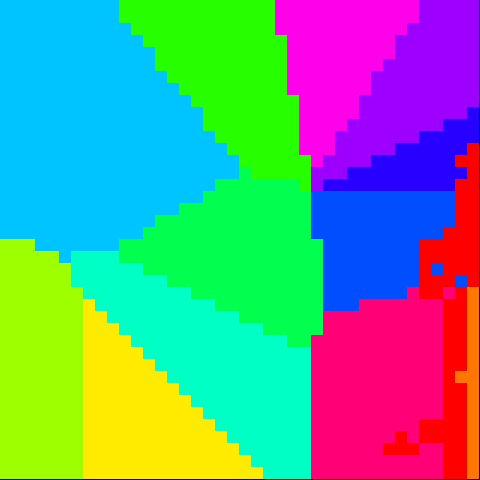
\includegraphics[width=40mm]{./g4012.png}}
\subfigure[16 semillas]{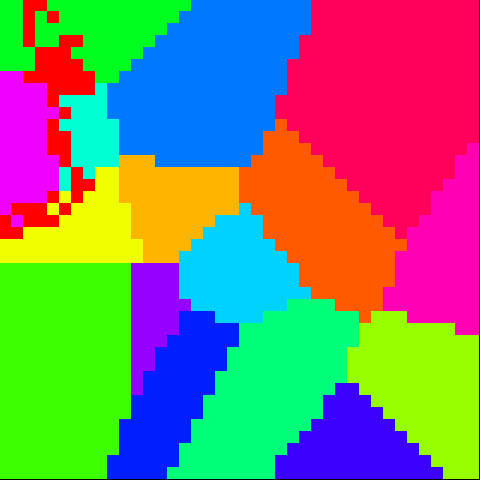
\includegraphics[width=40mm]{./g4016.png}}
\subfigure[20 semillas]{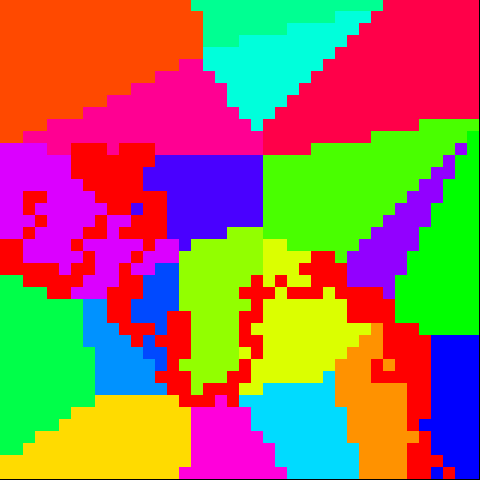
\includegraphics[width=40mm]{./g4020.png}}
\caption{Grietas en matríz 40x40 con diferente cantidad de semillas} \label{figura 4}
\end{figure}


\begin{figure}[htbp]
\centering
\subfigure[]{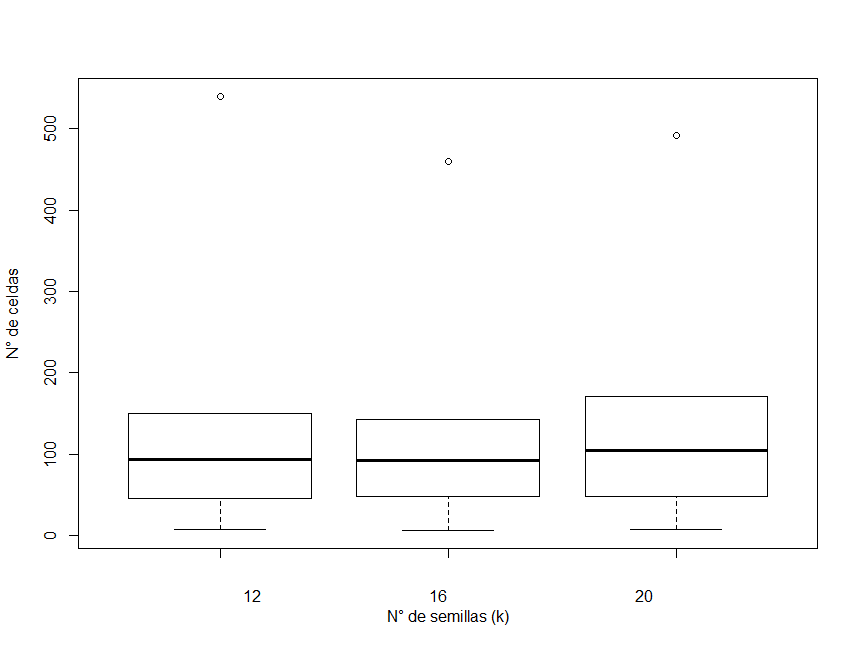
\includegraphics[width=80mm]{./celdas40.png}}
\subfigure[]{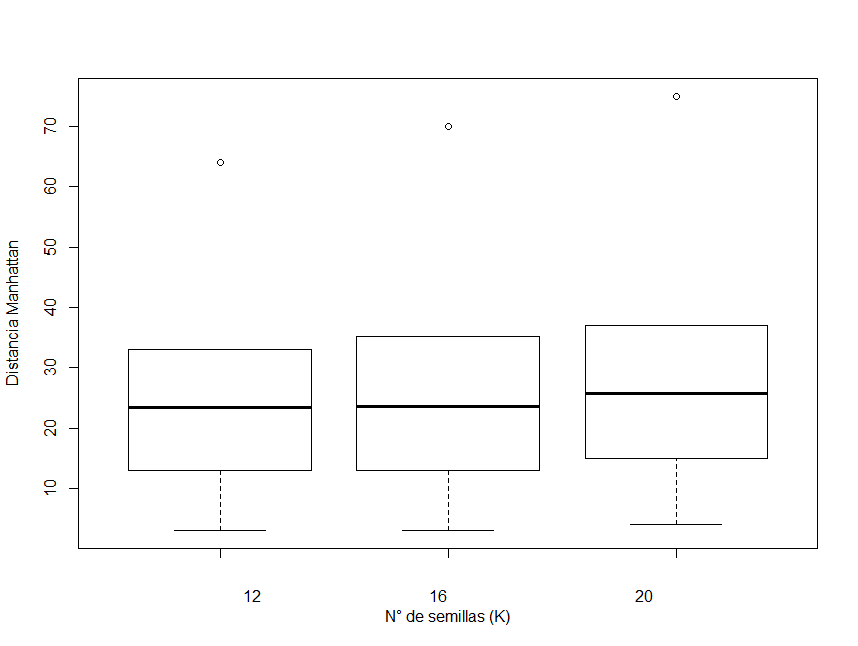
\includegraphics[width=80mm]{./dist40.png}}
\caption{Gráficas caja-bigote para número de celdas y distancia Manhattan vs. número de semillas en matríz de 40x40} \label{figura 1}
\end{figure}

Para la matríz 60x60 la grieta es grande \ref{figura 5} y profunda con un k de 20 pero aún está relativamente cerca de los límites de la matríz, siendo mas larga la distancia que la matríz 40x40 a la misma k \ref{figura 2}.

\begin{figure}[htbp]
\centering
\subfigure[12 semillas]{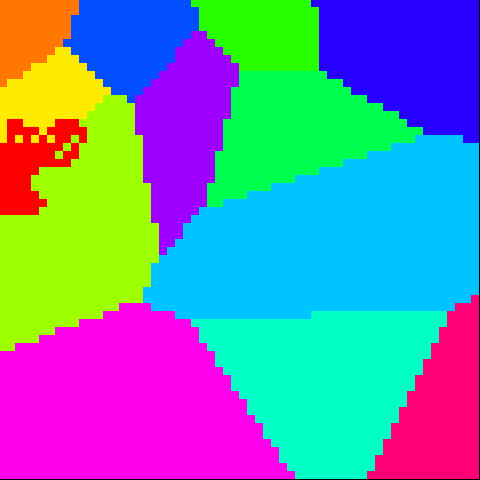
\includegraphics[width=40mm]{./g6012.png}}
\subfigure[16 semillas]{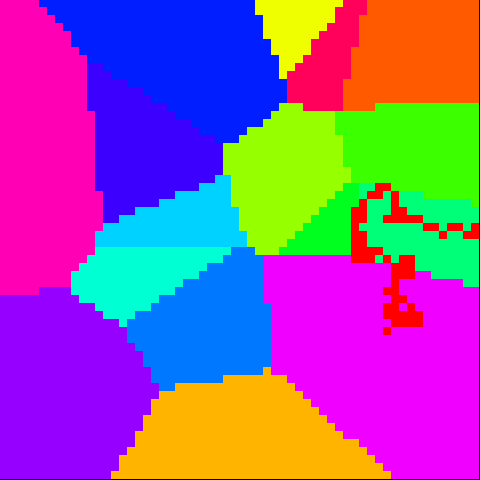
\includegraphics[width=40mm]{./g6016.png}}
\subfigure[20 semillas]{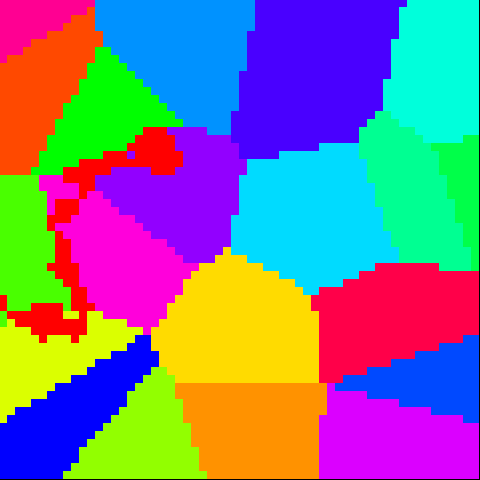
\includegraphics[width=40mm]{./g6020.png}}
\caption{Grietas en matríz 60x60 con diferente cantidad de semillas} \label{figura 5}
\end{figure}

\begin{figure}[htbp]
\centering
\subfigure[]{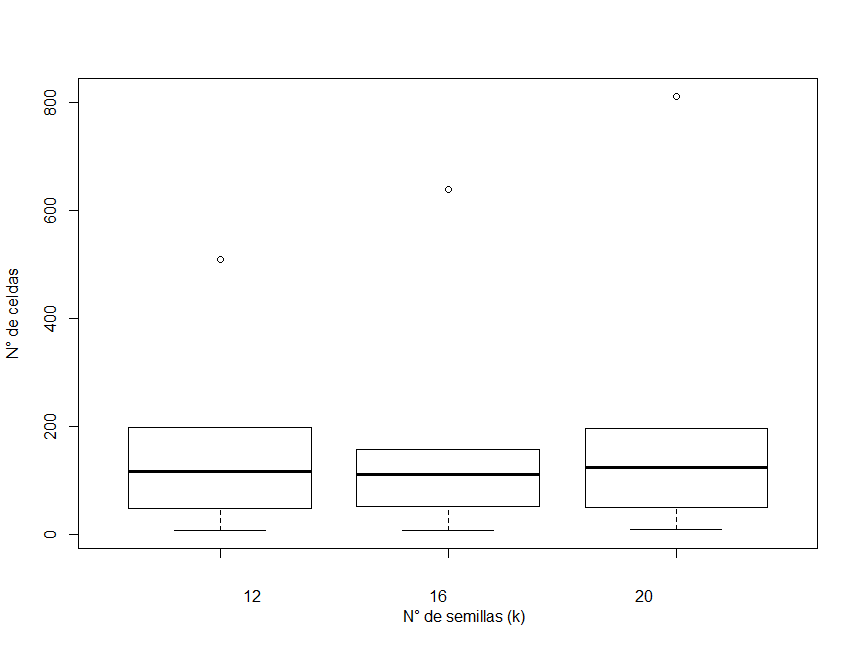
\includegraphics[width=80mm]{./celdas60.png}}
\subfigure[]{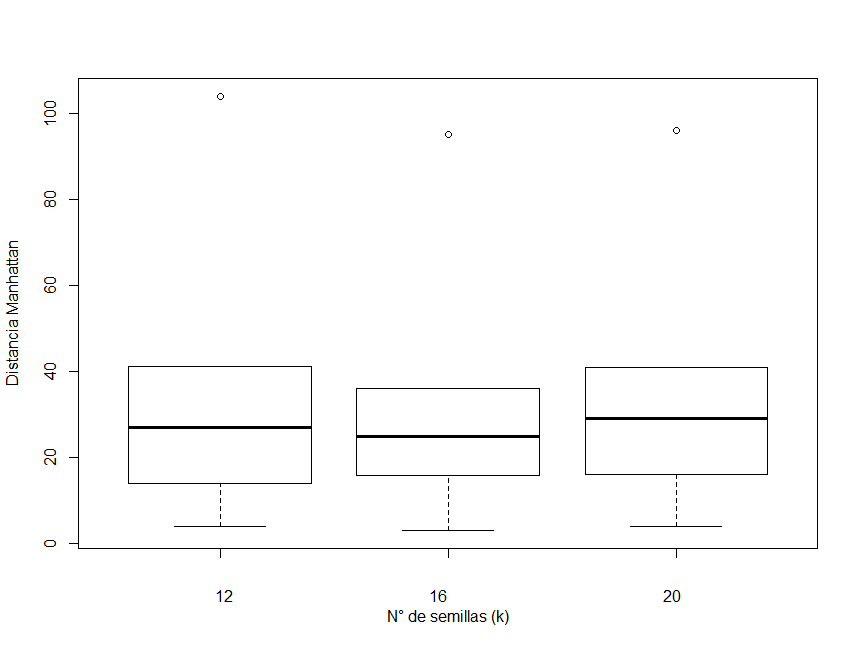
\includegraphics[width=80mm]{./dist60.png}}
\caption{Gráficas caja-bigote para número de celdas y distancia Manhattan vs. número de semillas en matríz de 60x60 } \label{figura 2}
\end{figure}

Para la matríz 80x80 se pueden observar grietas de mayor longitud \ref{figura 6} aun en un k de 12, se puede observar en las gráficas \ref{figura 3} que la distancia no varía mucho entre k=16 y k=20 aunque la cantidad de celdas ocupadas por la grieta sea grande.

\begin{figure}[htbp]
\centering
\subfigure[12 semillas]{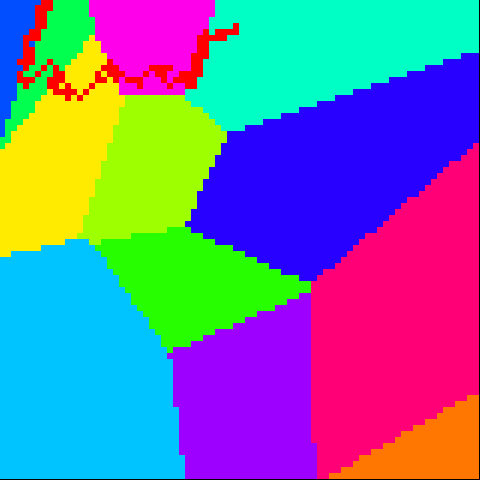
\includegraphics[width=40mm]{./g8012.png}}
\subfigure[16 semillas]{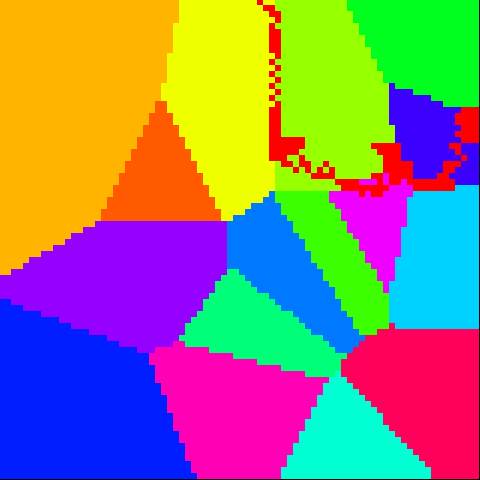
\includegraphics[width=40mm]{./g8016.png}}
\subfigure[20 semillas]{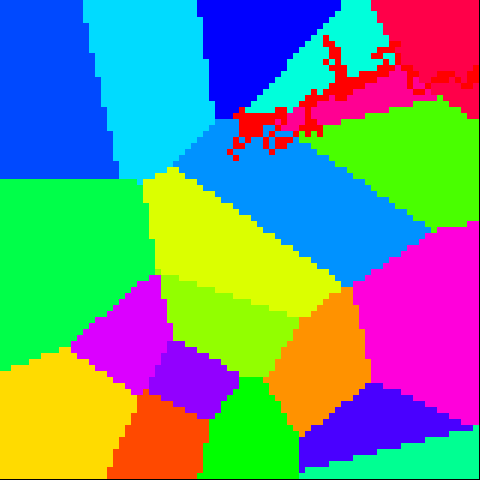
\includegraphics[width=40mm]{./g8020.png}}
\caption{Grietas en matríz 80x80 con diferente cantidad de semillas} \label{figura 6}
\end{figure}

\begin{figure}[htbp]
\centering
\subfigure[]{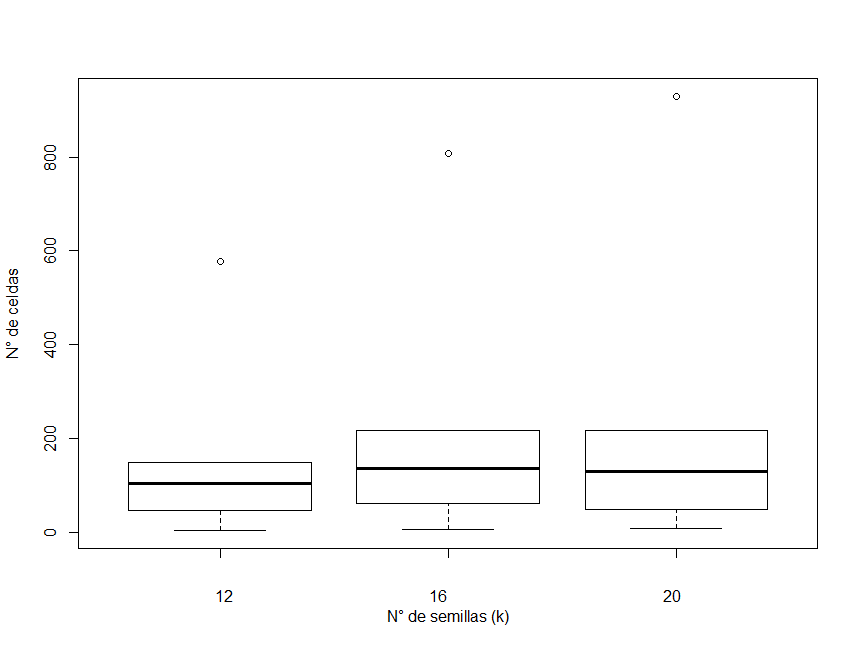
\includegraphics[width=80mm]{./celdas80.png}}
\subfigure[]{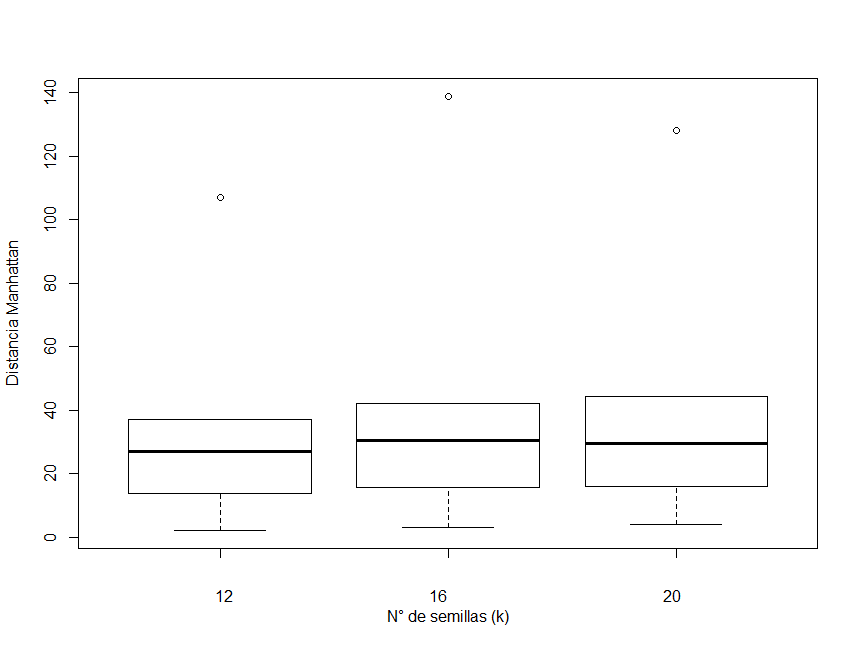
\includegraphics[width=80mm]{./dist80.png}}
\caption{Gráficas caja-bigote para número de celdas y distancia Manhattan vs. número de semillas en matríz de 80x80} \label{figura 3}
\end{figure}



\newpage

\section{Conclusiones}
De acuerdo con los resultados a una relación de menor n y mayor k en este caso 40 y 20, la grieta se propaga de manera más fácil hacia el centro de la matriz a causa de haber más fronteras por donde pasar y un espacio angosto en el cual crecer. Así mismo, a una relación de mayor n y menor k, en este caso 80 y 12, el tamaño de grieta y su propagación hacia el centro no son significativos, debido a que el espacio es demasiado amplio y hay menor cantidad de fronteras por las cuales la grieta pueda crecer.

\bibliographystyle{plainnat}
\bibliography{Bibliosimu}

\end{document}